\documentclass[conference]{IEEEtran}
\IEEEoverridecommandlockouts
\usepackage{cite}
\usepackage{amsmath,amssymb}
\usepackage{graphicx}
\usepackage{booktabs}
\usepackage{multirow}
\usepackage{tikz}
\usetikzlibrary{positioning,arrows.meta,fit,backgrounds}
\usepackage{url}

\begin{document}

\title{Multi-Aspect Sentiment Analysis of Product Reviews with R-Drop Regularized RoBERTa}

\author{
\IEEEauthorblockN{Deepanshu}
\IEEEauthorblockA{B.Tech CSAI\\Rishihood University}
\and
\IEEEauthorblockN{Agrapujya}
\IEEEauthorblockA{B.Tech CSAI\\Rishihood University}
\and
\IEEEauthorblockN{Kartik}
\IEEEauthorblockA{B.Tech CSAI\\Rishihood University}
\and
\IEEEauthorblockN{Sahil}
\IEEEauthorblockA{B.Tech CSAI\\Rishihood University}
}

\maketitle

\begin{abstract}
A single star rating hides the mixed opinions inside a product review. We present a system that extracts every aspect a review mentions, assigns each its own sentiment, and summarises many reviews as Amazon-style ``Customers say'' aspect chips. Aspect extraction and sentiment are learned jointly as 7-label BIO token classification. We compare five encoders---BERT, RoBERTa, DeBERTa-v3, ModernBERT, and RoBERTa with R-Drop consistency regularisation---under one protocol on the official SemEval-2014 Task~4 test sets, with three seeds and equal training budgets. RoBERTa with R-Drop achieves the best strict end-to-end F1, $68.89\pm0.20$ on laptops and $78.90\pm0.25$ on restaurants, beating plain RoBERTa on every seed in both domains and statistically tying DeBERTa-v3 at half its training cost. We also report an in-depth review of the original project, which identified five problems: evaluation on a slice of the training data, the silent loss of 44\% of sentences, single-seed comparisons, spelling-only aspect grouping, and silent truncation of long reviews. We describe how each was fixed: meaning-based grouping with sentence embeddings raises grouping F1 from 0.20 to 0.87, and sentence-boundary chunking removes the truncation without changing outputs on short reviews. Code, results, and the trained model are publicly released.
\end{abstract}

\begin{IEEEkeywords}
aspect-based sentiment analysis, token classification, R-Drop, RoBERTa, opinion summarization, SemEval-2014
\end{IEEEkeywords}

%=====================================================================
\section{Introduction}
Online shoppers increasingly rely on reviews, but a five-star scale compresses opinions about many product features into one number. A three-star review may praise the battery and condemn the case. \emph{Aspect-based sentiment analysis} (ABSA) recovers this detail by identifying what is being discussed (the \emph{aspect}, e.g., ``battery life'') and how the writer feels about it. E-commerce platforms surface the result as aspect summaries; Amazon introduced AI-generated ``Customers say'' highlights with clickable aspect chips in 2023.

We address \emph{end-to-end} ABSA (E2E-ABSA), which extracts aspect terms and their polarity jointly~\cite{li2019bert}, and build it into a complete review-summarisation pipeline. The project began from an open-source prototype that trained five encoders on SemEval-2014 and served the best one in a web interface. An in-depth review revealed that its evaluation could not support its conclusions, and that the product pipeline had silent failure modes. This report presents the system, the review, and the fixes.

Our contributions are:
\begin{itemize}
\item A controlled comparison of five transformer encoders for E2E-ABSA on the official SemEval-2014 test sets, with three seeds, equal epochs, and character-level strict metrics.
\item Evidence that R-Drop~\cite{liang2021rdrop} consistently improves RoBERTa for E2E-ABSA (+1.42 F1 on laptops, +1.04 on restaurants, winning all 3 seeds), at zero inference cost.
\item A meaning-based aspect-grouping method using sentence embeddings, phrase normalisation, and agglomerative clustering, raising grouping F1 from 0.20 to 0.87.
\item Sentence-boundary chunking for reviews beyond the encoder's 512-token window, without altering results on shorter reviews.
\item A documented review of the original project's evaluation and engineering, with each issue traced to a measured fix.
\end{itemize}

%=====================================================================
\section{Related Work}
\textbf{E2E-ABSA.} Li et~al.~\cite{li2019bert} cast E2E-ABSA as unified sequence tagging on BERT, reporting 60.4--61.1 F1 on the SemEval-2014 laptop set. Hu et~al.~\cite{hu2019span} proposed span-based extract-then-classify models. GRACE~\cite{luo2020grace} adds cascaded labelling and post-training (70.7 F1 on laptops). Generative approaches cast the task as sequence generation: BARTABSA~\cite{yan2021unified} and GAS~\cite{zhang2021gas}; instruction-tuned InstructABSA~\cite{scaria2023instructabsa} reports about 79 F1 on both domains.

\textbf{Large language models.} Zero-shot ChatGPT reaches only 33.1 (laptop) and 54.5 (restaurant) exact-match F1 on E2E-ABSA~\cite{zhang2023llm}, far below fine-tuned encoders, largely due to span-boundary mismatches.

\textbf{Encoders and regularisation.} We compare BERT~\cite{devlin2019bert}, RoBERTa~\cite{liu2019roberta}, DeBERTa-v3~\cite{he2023debertav3}, and ModernBERT~\cite{warner2024modernbert}, a 2024 encoder with an 8,192-token context. R-Drop~\cite{liang2021rdrop} regularises dropout by penalising the divergence between two stochastic forward passes, improving GLUE by about 1.2 points for BERT-base.

\textbf{Evaluation reliability.} Fine-tuning results vary substantially with the random seed~\cite{reimers2017reporting,dodge2020finetuning}, so single-seed comparisons of about one point are unreliable. Removing sentences without aspects inflates E2E-ABSA F1 by about 5 points~\cite{gong2020unified}. SemEval-2014 is also known to under-represent sentences with conflicting sentiments~\cite{jiang2019mams,xing2020arts}.

%=====================================================================
\section{Dataset}
We use SemEval-2014 Task~4~\cite{pontiki2014semeval}, laptop and restaurant domains, from the original XML release (a pinned Hugging Face copy). The counts match the official release exactly: 3,045 and 3,041 training sentences, and 800 and 800 test sentences. About 40\% of sentences contain no aspect; these are retained so that the model learns when to predict nothing. Aspects labelled \emph{conflict} are excluded: training and development sentences containing one are dropped, while every test sentence is kept with conflict spans unlabelled, following~\cite{li2019bert}. Each domain's official training set is split 90/10 into train and dev with one fixed split for all runs; scores are computed only on the official gold test sets. Table~\ref{tab:data} summarises the splits.

\begin{table}[t]
\caption{Dataset statistics (sentences and aspect polarities)}
\label{tab:data}
\centering
\setlength{\tabcolsep}{4pt}
\begin{tabular}{@{}lrrrrrr@{}}
\toprule
Split & Sent. & No asp. & Aspects & Pos & Neg & Neu \\
\midrule
Train (90\%)       & 5,346 & 2,302 & 5,221 & 2,798 & 1,462 & 961 \\
Dev (10\%)         &   595 &   265 &   585 &   297 &   168 & 120 \\
Test, laptops      &   800 &   389 &   638 &   341 &   128 & 169 \\
Test, restaurants  &   800 &   200 & 1,120 &   728 &   196 & 196 \\
\bottomrule
\end{tabular}
\end{table}

%=====================================================================
\section{Methodology}

\subsection{Problem Formulation}
Given a sentence $x=(x_1,\dots,x_n)$ of sub-word tokens, the model predicts one label per token from
\begin{equation}
\mathcal{Y}=\{\texttt{O}\}\cup\{\texttt{B},\texttt{I}\}\times\{\texttt{POS},\texttt{NEG},\texttt{NEU}\},
\end{equation}
giving 7 labels. \texttt{B} marks the first token of an aspect and \texttt{I} its continuation; the polarity is carried by the tag. For example, ``The battery life is great but the charging case feels cheap'' is tagged \texttt{O B-POS I-POS O O O O B-NEG I-NEG O O}. Aspect extraction and polarity classification are thus learned jointly by a token-classification head on a pretrained encoder. Gold character spans are projected onto tokens via the tokenizer's offset mapping, and the projection is lossless in practice: 1,756 of 1,758 test aspects round-trip exactly.

\subsection{R-Drop Regularisation}
Each training batch is passed through the network twice, yielding two predictive distributions $p_1$ and $p_2$ that differ only through dropout. With token cross-entropy $\mathcal{L}_{CE}$ over non-padding tokens, the loss is
\begin{equation}
\begin{split}
\mathcal{L} ={}& \tfrac{1}{2}\big(\mathcal{L}_{CE}(p_1)+\mathcal{L}_{CE}(p_2)\big)\\
&+ \alpha\cdot\tfrac{1}{2}\big(D_{KL}(p_1\Vert p_2)+D_{KL}(p_2\Vert p_1)\big),
\end{split}
\end{equation}
with $\alpha=1.5$. R-Drop roughly doubles training compute and leaves inference unchanged.

\subsection{Decoding and Long Reviews}
Predicted tags are decoded into character spans; an \texttt{I} tag without a preceding aspect of the same polarity starts a new span, and each span's confidence is its mean token probability. A review that fits the 512-token window is tagged in one pass. Longer reviews are segmented at sentence boundaries and the sentences are greedily packed into chunks that fit; a single over-long sentence is split into token windows. Span offsets are mapped back to the full review, so no text is dropped.

\subsection{Aspect Grouping}
To build chips, mentions across reviews are grouped as follows (Fig.~\ref{fig:pipeline}):
\begin{enumerate}
\item \emph{Normalisation:} lowercasing, removal of leading determiners, simple singularisation with exceptions, and stripping of attribute words (\emph{life}, \emph{quality}, \emph{level}), e.g., ``The Battery life'' $\rightarrow$ ``battery''.
\item \emph{Embedding:} each normalised phrase is embedded in the template ``The product's \{aspect\}.'' with the pretrained sentence encoder all-MiniLM-L6-v2~\cite{reimers2019sbert,wang2020minilm} (mean pooling, unit norm). No training is required.
\item \emph{Clustering:} average-linkage agglomerative clustering with a cosine-distance threshold of 0.25. Each cluster becomes a chip named by its most frequent surface form, with positive, negative, and neutral counts.
\end{enumerate}
If the embedding model is unavailable (e.g., offline), the system falls back to exact matching of normalised phrases.

\begin{figure*}[t]
\centering
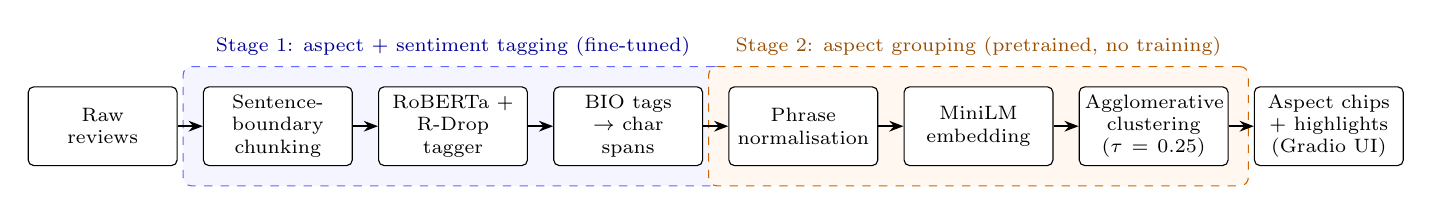
\begin{tikzpicture}[font=\scriptsize, node distance=3.2mm,
  box/.style={draw, rounded corners=2pt, align=center, minimum height=10mm, text width=17.5mm, inner sep=2pt, fill=white},
  arr/.style={-{Stealth[length=1.8mm]}, thick}]
\node[box] (a) {Raw\\reviews};
\node[box, right=of a] (b) {Sentence-\\boundary\\chunking};
\node[box, right=of b] (c) {RoBERTa +\\R-Drop\\tagger};
\node[box, right=of c] (d) {BIO tags\\$\rightarrow$ char\\spans};
\node[box, right=of d] (e) {Phrase\\normalisation};
\node[box, right=of e] (f) {MiniLM\\embedding};
\node[box, right=of f] (g) {Agglomerative\\clustering\\($\tau=0.25$)};
\node[box, right=of g] (h) {Aspect chips\\+ highlights\\(Gradio UI)};
\foreach \x/\y in {a/b,b/c,c/d,d/e,e/f,f/g,g/h} \draw[arr] (\x)--(\y);
\begin{scope}[on background layer]
\node[draw=blue!60, dashed, rounded corners=3pt, fill=blue!4, fit=(b)(c)(d), inner sep=2.5mm, label={[font=\scriptsize, text=blue!60!black]above:Stage 1: aspect + sentiment tagging (fine-tuned)}] {};
\node[draw=orange!80!black, dashed, rounded corners=3pt, fill=orange!6, fit=(e)(f)(g), inner sep=2.5mm, label={[font=\scriptsize, text=orange!60!black]above:Stage 2: aspect grouping (pretrained, no training)}] {};
\end{scope}
\end{tikzpicture}
\caption{System pipeline. Stage~1 jointly extracts aspects and their sentiment with a fine-tuned encoder; Stage~2 groups mentions across reviews by meaning into summary chips.}
\label{fig:pipeline}
\end{figure*}

%=====================================================================
\section{Experimental Setup}
All encoders are base-size checkpoints fine-tuned with the Hugging Face Transformers library~\cite{wolf2020transformers}, using the hyper-parameters in Table~\ref{tab:hparams}. All models train for 6 epochs; the checkpoint with the best dev F1 is evaluated. DeBERTa-v3 is trained in fp32 because of reported fp16 instability; the others use fp16. Each configuration is run with seeds 42, 43, and 44 (15 runs) on a single NVIDIA T4 GPU (Kaggle), taking about one hour in total.

\begin{table}[t]
\caption{Training configuration}
\label{tab:hparams}
\centering
\setlength{\tabcolsep}{4pt}
\begin{tabular}{@{}lrrcr@{}}
\toprule
Model & Params & LR & Precision & Min/seed \\
\midrule
BERT-base         & 109M & 3e-5 & fp16 & 2.3 \\
RoBERTa-base      & 124M & 3e-5 & fp16 & 2.4 \\
DeBERTa-v3-base   & 184M & 2e-5 & fp32 & 7.3 \\
ModernBERT-base   & 150M & 3e-5 & fp16 & 3.7 \\
RoBERTa + R-Drop  & 124M & 3e-5 & fp16 & 3.9 \\
\midrule
\multicolumn{5}{@{}l@{}}{\footnotesize Shared: batch 16, 6 epochs, weight decay 0.01, 10\% warmup,}\\
\multicolumn{5}{@{}l@{}}{\footnotesize gradient clip 1.0, max length 256, R-Drop $\alpha=1.5$.}\\
\bottomrule
\end{tabular}
\end{table}

\textbf{Metrics.} The primary metric is \emph{strict} E2E micro-F1: a predicted aspect is correct only if its character span and polarity both match the gold annotation exactly. We also report span-only (aspect term extraction) F1, per-polarity F1, macro-F1 over the three polarities, and the \emph{false-aspect rate}: the fraction of aspect-free test sentences in which any aspect is predicted.

%=====================================================================
\section{Results}

\subsection{Main Comparison}
Table~\ref{tab:main} and Fig.~\ref{fig:results} report strict E2E-F1 on the official test sets. RoBERTa with R-Drop obtains the best mean in both domains and the smallest variance across seeds. Against plain RoBERTa it wins on all three seeds in both domains, with per-seed gains of $+1.07$, $+2.56$, $+0.64$ (laptops) and $+0.12$, $+1.33$, $+1.66$ (restaurants), so the improvement exceeds seed noise. Its lead over DeBERTa-v3 ($+0.63$ and $+0.29$) is smaller than DeBERTa's own standard deviation; we therefore regard the two as tied, with R-Drop training in about half the time. In an earlier throughput test on the same GPU, RoBERTa variants processed about 1,560 sentences/s against 281 for DeBERTa-v3, though DeBERTa ran in fp32.

\begin{table}[t]
\caption{Strict E2E-F1 (\%) on the official SemEval-2014 test sets, mean $\pm$ std over 3 seeds}
\label{tab:main}
\centering
\setlength{\tabcolsep}{3.5pt}
\begin{tabular}{@{}lccc@{}}
\toprule
Model & Laptop14 & Rest14 & Pooled \\
\midrule
BERT-base         & 59.71 $\pm$ 0.31 & 73.24 $\pm$ 0.64 & 68.34 $\pm$ 0.48 \\
ModernBERT-base   & 59.45 $\pm$ 1.35 & 74.17 $\pm$ 0.47 & 68.86 $\pm$ 0.76 \\
RoBERTa-base      & 67.47 $\pm$ 0.81 & 77.86 $\pm$ 0.56 & 74.11 $\pm$ 0.48 \\
DeBERTa-v3-base   & 68.26 $\pm$ 0.82 & 78.61 $\pm$ 1.33 & 74.84 $\pm$ 1.03 \\
\textbf{RoBERTa + R-Drop} & \textbf{68.89 $\pm$ 0.20} & \textbf{78.90 $\pm$ 0.25} & \textbf{75.29 $\pm$ 0.21} \\
\bottomrule
\end{tabular}
\end{table}

\begin{figure}[t]
\centering
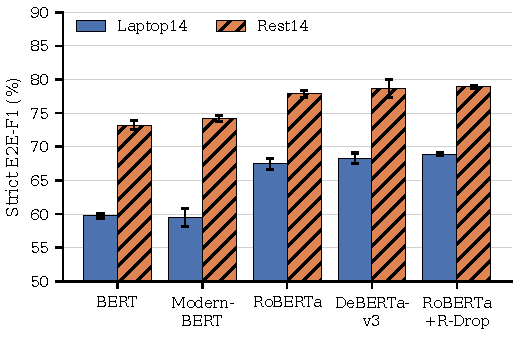
\includegraphics[width=\columnwidth]{fig_results.pdf}
\caption{Strict E2E-F1 per domain; error bars show the standard deviation over three seeds.}
\label{fig:results}
\end{figure}

\subsection{Error Analysis}
For RoBERTa + R-Drop on the pooled test set, span-only F1 is 0.862 while strict F1 is 0.753, so most errors concern polarity rather than locating the aspect. Per-polarity F1 is 0.824 (positive), 0.713 (negative), and 0.555 (neutral); macro-F1 is 0.697. Neutral is clearly the weakest class for every encoder (Fig.~\ref{fig:polarity}), likely because neutral aspects are the rarest in training (961 of 5,221) and often carry no explicit opinion word. On aspect-free test sentences the model predicts a spurious aspect in 4.8\% of laptop and 9.3\% of restaurant cases. ModernBERT's weak laptop score likely reflects its untuned learning rate: we used the shared 3e-5, while its maintainers recommend 3e-5 to 1e-4.

\begin{figure}[t]
\centering
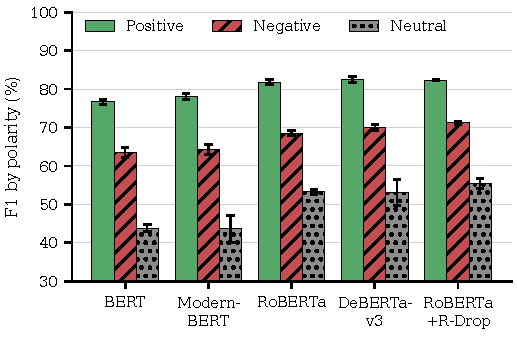
\includegraphics[width=\columnwidth]{fig_polarity.pdf}
\caption{F1 by polarity on the pooled test sets (mean $\pm$ std over three seeds). Neutral lags positive and negative for every encoder.}
\label{fig:polarity}
\end{figure}

\subsection{Comparison with Published Work}
Table~\ref{tab:lit} places our results among published E2E-ABSA systems. Our BERT baseline (59.7) reproduces Li et~al.~\cite{li2019bert} (60.4--61.1), validating the pipeline. RoBERTa + R-Drop matches GAS~\cite{zhang2021gas} and exceeds BARTABSA~\cite{yan2021unified}, but trails GRACE~\cite{luo2020grace} on laptops and InstructABSA~\cite{scaria2023instructabsa}. Unlike most published systems, we train a single model on both domains and average three rather than 5--10 seeds. All fine-tuned systems outperform zero-shot ChatGPT~\cite{zhang2023llm} by roughly 10--30 points.

\begin{table}[t]
\caption{Comparison with published E2E-ABSA results (F1, \%)}
\label{tab:lit}
\centering
\setlength{\tabcolsep}{4pt}
\begin{tabular}{@{}lcc@{}}
\toprule
Method & Laptop14 & Rest14 \\
\midrule
ChatGPT, zero-shot~\cite{zhang2023llm} & 33.1 & 54.5 \\
BERT + linear/CRF~\cite{li2019bert} & 60.4--61.1 & 73.2--74.7$^{*}$ \\
BARTABSA~\cite{yan2021unified} & 67.4 & 73.6 \\
GAS, T5-base~\cite{zhang2021gas} & 68.1 & 77.1 \\
GRACE~\cite{luo2020grace} & 70.7 & 77.3$^{*}$ \\
InstructABSA~\cite{scaria2023instructabsa} & 79.3 & 79.5 \\
\midrule
Ours: BERT-base & 59.7 & 73.2 \\
Ours: RoBERTa + R-Drop & 68.9 & 78.9 \\
\bottomrule
\multicolumn{3}{@{}l@{}}{\footnotesize $^{*}$Restaurant data of SemEval 2014--2016 combined.}
\end{tabular}
\end{table}

\subsection{Aspect Grouping}
We evaluate grouping on a held-out set of 68 aspect phrases in 30 gold groups, written before any tuning; it includes hard negatives such as \emph{screen}/\emph{screen protector}. Table~\ref{tab:group} reports pairwise precision, recall, and F1. The original method, clustering the tagger's embedding-layer vectors, captures spelling but not meaning: it merges only 11\% of true synonym pairs. Our method reaches 0.87 F1 at the pre-registered threshold of 0.25. Its only wrong merge joins \emph{earbuds} with the \emph{ear cushions} group; a stricter threshold of 0.20 removes it at the cost of recall. Fig.~\ref{fig:grouping} shows the full precision--recall trade-off: F1 peaks at 0.893 at $\tau=0.225$, but we keep the threshold fixed before evaluation rather than tune it on the held-out set.

\begin{figure}[t]
\centering
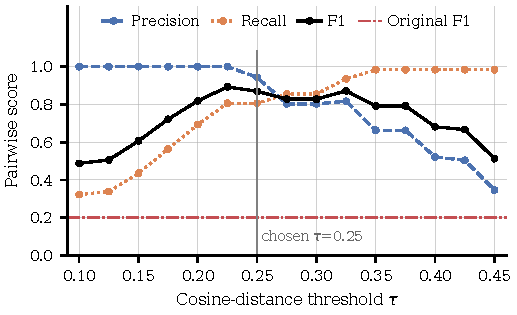
\includegraphics[width=\columnwidth]{fig_grouping.pdf}
\caption{Aspect-grouping precision, recall, and F1 versus the clustering threshold $\tau$ on 68 held-out phrases. The dash-dotted line is the original method's F1 (0.20).}
\label{fig:grouping}
\end{figure}

\begin{table}[t]
\caption{Aspect-grouping quality on 68 held-out phrases}
\label{tab:group}
\centering
\begin{tabular}{@{}lcccc@{}}
\toprule
Method & P & R & F1 & ARI \\
\midrule
Embedding layer, $\tau=0.22$ (original) & 1.00 & 0.11 & 0.20 & 0.20 \\
Ours, $\tau=0.20$ & 1.00 & 0.69 & 0.82 & 0.81 \\
\textbf{Ours, $\tau=0.25$} & \textbf{0.94} & \textbf{0.81} & \textbf{0.87} & \textbf{0.87} \\
Ours, $\tau=0.30$ & 0.80 & 0.85 & 0.83 & 0.82 \\
\bottomrule
\end{tabular}
\end{table}

\subsection{Qualitative Behaviour}
On electronics reviews outside the training domains (headphones, laptops), the model is mostly correct with high confidence, e.g., \emph{noise cancellation} (positive, 1.00), \emph{ear cushions} (negative, 1.00). Systematic failures remain on expectation reversals (``I expected the battery to be terrible, but it is excellent'' $\rightarrow$ negative, 0.90) and idioms (``The battery dies fast'' $\rightarrow$ positive, 0.99), and on one demo sentence (``the charging case feels cheap'' $\rightarrow$ positive, 0.81).

%=====================================================================
\section{Review of the Original Project}
Table~\ref{tab:review} summarises the issues identified in the original prototype and how each was resolved. The most consequential were in evaluation. The prototype loaded a per-aspect copy of the data in which sentences without aspects cannot appear, discarding 44\% of the training sentences. It then evaluated on a random 10\% of the \emph{training} data rather than the official test sets, using one seed, and gave R-Drop one more epoch than the baselines. Under that protocol R-Drop's +1.2 F1 lead was within seed noise. Under the corrected protocol, the lead over RoBERTa holds on every seed. Contrary to our expectation, scores rose rather than fell (pooled 75.3 vs.\ 69.2), most likely because restoring the missing sentences roughly doubled the training data.

\begin{table}[t]
\caption{Issues found in the original project and their resolution}
\label{tab:review}
\centering
\footnotesize
\setlength{\tabcolsep}{3pt}
\begin{tabular}{@{}p{0.43\columnwidth}p{0.53\columnwidth}@{}}
\toprule
Issue & Resolution and evidence \\
\midrule
Tested on a slice of training data & Official test sets, per domain \\
44\% of sentences (no aspect) lost & Original XML; counts match release \\
Single seed; unequal epochs & 3 seeds, 6 epochs for all models \\
Synonyms never grouped & MiniLM grouping: F1 0.20 $\rightarrow$ 0.87 \\
Reviews truncated at 512 tokens & Sentence chunking; short reviews unchanged (35/35 spans identical) \\
Path depended on working directory & Resolved relative to repository \\
Failed model load cached forever & Failures retried \\
No README, tests, or public weights & README, 41 tests, weights on the Hub \\
\bottomrule
\end{tabular}
\end{table}

%=====================================================================
\section{Limitations and Future Work}
Neutral sentiment remains weak (F1 0.555), suggesting class re-weighting or targeted data. Sentences that reverse an expectation, and idioms, call for training and evaluation on contrast sets such as MAMS~\cite{jiang2019mams} and ARTS~\cite{xing2020arts}. The model was trained only on laptops and restaurants and has not been evaluated on labelled reviews from the target product domains; a small in-domain labelled set is the most direct next step. Spurious aspects (5--9\% of aspect-free sentences) could be reduced by confidence calibration and a minimum-support rule for chips. Finally, settling R-Drop against DeBERTa-v3 needs more seeds and an $\alpha$ sweep, and ModernBERT deserves its own learning-rate search.

%=====================================================================
\section{Conclusion}
We built an end-to-end aspect-based sentiment system that turns raw reviews into Amazon-style aspect summaries. Under a corrected, multi-seed protocol on the official SemEval-2014 test sets, RoBERTa with R-Drop is the most accurate and most stable of five encoders, reaching 68.89 (laptops) and 78.90 (restaurants) strict F1. It reproduces the established BERT baseline and matches 2021-era research systems. Meaning-based grouping and sentence-level chunking make the pipeline robust for real reviews. The review of the original prototype shows that the evaluation protocol, not the model, was the main obstacle to trustworthy conclusions.

\section*{Code and Model Availability}
{\raggedright\small
Code: \url{https://github.com/antedotee/nlp-multi-aspect-analyzer}\\
Branch: \texttt{improve/official-benchmark-and-fixes}\\
Model: \url{https://huggingface.co/Deepanshu027/roberta-base-rdrop-absa-semeval14}\par}

%=====================================================================
\begin{thebibliography}{00}
\bibitem{pontiki2014semeval} M. Pontiki, D. Galanis, J. Pavlopoulos, H. Papageorgiou, I. Androutsopoulos, and S. Manandhar, ``SemEval-2014 Task 4: Aspect based sentiment analysis,'' in \emph{Proc. 8th Int. Workshop on Semantic Evaluation (SemEval)}, 2014, pp. 27--35.
\bibitem{li2019bert} X. Li, L. Bing, W. Zhang, and W. Lam, ``Exploiting BERT for end-to-end aspect-based sentiment analysis,'' in \emph{Proc. 5th Workshop on Noisy User-generated Text (W-NUT)}, 2019, pp. 34--41.
\bibitem{hu2019span} M. Hu, Y. Peng, Z. Huang, D. Li, and Y. Lv, ``Open-domain targeted sentiment analysis via span-based extraction and classification,'' in \emph{Proc. ACL}, 2019, pp. 537--546.
\bibitem{luo2020grace} H. Luo, L. Ji, T. Li, D. Jiang, and N. Duan, ``GRACE: Gradient harmonized and cascaded labeling for aspect-based sentiment analysis,'' in \emph{Findings of EMNLP}, 2020, pp. 54--64.
\bibitem{yan2021unified} H. Yan, J. Dai, T. Ji, X. Qiu, and Z. Zhang, ``A unified generative framework for aspect-based sentiment analysis,'' in \emph{Proc. ACL-IJCNLP}, 2021, pp. 2416--2429.
\bibitem{zhang2021gas} W. Zhang, X. Li, Y. Deng, L. Bing, and W. Lam, ``Towards generative aspect-based sentiment analysis,'' in \emph{Proc. ACL-IJCNLP (Short Papers)}, 2021, pp. 504--510.
\bibitem{scaria2023instructabsa} K. Scaria, H. Gupta, S. Goyal, S. A. Sawant, S. Mishra, and C. Baral, ``InstructABSA: Instruction learning for aspect based sentiment analysis,'' arXiv:2302.08624, 2023.
\bibitem{zhang2023llm} W. Zhang, Y. Deng, B. Liu, S. J. Pan, and L. Bing, ``Sentiment analysis in the era of large language models: A reality check,'' arXiv:2305.15005, 2023.
\bibitem{devlin2019bert} J. Devlin, M.-W. Chang, K. Lee, and K. Toutanova, ``BERT: Pre-training of deep bidirectional transformers for language understanding,'' in \emph{Proc. NAACL-HLT}, 2019, pp. 4171--4186.
\bibitem{liu2019roberta} Y. Liu \emph{et al.}, ``RoBERTa: A robustly optimized BERT pretraining approach,'' arXiv:1907.11692, 2019.
\bibitem{he2023debertav3} P. He, J. Gao, and W. Chen, ``DeBERTaV3: Improving DeBERTa using ELECTRA-style pre-training with gradient-disentangled embedding sharing,'' in \emph{Proc. ICLR}, 2023.
\bibitem{warner2024modernbert} B. Warner \emph{et al.}, ``Smarter, better, faster, longer: A modern bidirectional encoder for fast, memory efficient, and long context finetuning and inference,'' arXiv:2412.13663, 2024.
\bibitem{liang2021rdrop} X. Liang \emph{et al.}, ``R-Drop: Regularized dropout for neural networks,'' in \emph{Advances in Neural Information Processing Systems (NeurIPS)}, 2021.
\bibitem{reimers2019sbert} N. Reimers and I. Gurevych, ``Sentence-BERT: Sentence embeddings using Siamese BERT-networks,'' in \emph{Proc. EMNLP-IJCNLP}, 2019, pp. 3982--3992.
\bibitem{wang2020minilm} W. Wang, F. Wei, L. Dong, H. Bao, N. Yang, and M. Zhou, ``MiniLM: Deep self-attention distillation for task-agnostic compression of pre-trained transformers,'' in \emph{Advances in Neural Information Processing Systems (NeurIPS)}, 2020.
\bibitem{reimers2017reporting} N. Reimers and I. Gurevych, ``Reporting score distributions makes a difference: Performance study of LSTM-networks for sequence tagging,'' in \emph{Proc. EMNLP}, 2017, pp. 338--348.
\bibitem{dodge2020finetuning} J. Dodge, G. Ilharco, R. Schwartz, A. Farhadi, H. Hajishirzi, and N. Smith, ``Fine-tuning pretrained language models: Weight initializations, data orders, and early stopping,'' arXiv:2002.06305, 2020.
\bibitem{gong2020unified} C. Gong, J. Yu, and R. Xia, ``Unified feature and instance based domain adaptation for aspect-based sentiment analysis,'' in \emph{Proc. EMNLP}, 2020, pp. 7035--7045.
\bibitem{jiang2019mams} Q. Jiang, L. Chen, R. Xu, X. Ao, and M. Yang, ``A challenge dataset and effective models for aspect-based sentiment analysis,'' in \emph{Proc. EMNLP-IJCNLP}, 2019, pp. 6280--6285.
\bibitem{xing2020arts} X. Xing \emph{et al.}, ``Tasty burgers, soggy fries: Probing aspect robustness in aspect-based sentiment analysis,'' in \emph{Proc. EMNLP}, 2020, pp. 3594--3605.
\bibitem{wolf2020transformers} T. Wolf \emph{et al.}, ``Transformers: State-of-the-art natural language processing,'' in \emph{Proc. EMNLP: System Demonstrations}, 2020, pp. 38--45.
\end{thebibliography}

\end{document}
